\section{BON extraction}
The textual \textsc{bon} extractor is a static analysis tool that provides an overview of a program written in Eiffel. Its purpose is to enable the user to benefits from the features of the textual \textsc{bon} language without having to leave an Eiffel development environment. Without having to write the textual \textsc{bon}.
\begin{figure}[H]
\centering
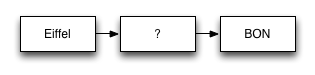
\includegraphics[scale=0.8]{images/BON-extraction-model-1.png}
\caption{BON Extraction Model 1}
\label{fig:bon_extraction_1}
\end{figure}
\label{design-bon-extraction}
Conceptually, the objective of the extractor is to bridge the gap between the Eiffel universe and the textual \textsc{bon} universe, as shown in figure \ref{fig:bon_extraction_1}. It does so by allowing the user to switch from an Eiffel-related view to either a formal or an informal textual \textsc{bon} view. When switching view, the user is presented to a textual \textsc{bon} representation of the Eiffel code. To add further overview over the system, the extractor also analyzes the descendants of the chosen class.

\subsection{Overall architecture}
The textual \textsc{bon} extractor has two main parts. One is the interface to EiffelStudio, the other is an internal representation of the \textsc{bon} language. Each of the two parts are independent and changes can be done in one without it having any effect on the other. With the exception of creation calls from the interface that hook into the internal representation.

\paragraph{}
For generating textual \textsc{bon},  an internal representation of \textsc{bon} has been created. This representation has a MOG-like structure with classes representing most of the \textsc{bon} elements defined in the grammar in \cite{walden1995}, with a few exceptions (See section \ref{deviations_from_bon}).  Each of these classes contains meta-information about the element, and knows how itself into format textual \textsc{bon} (both formal and informal) based on this information.

\subsubsection{From EiffelStudio to BON}
To bridge the aforementioned gap between EiffelStudio and the internal \textsc{bon} representation, an interface linking the two parts is needed. This interface needs be able to take input from EiffelStudio, and hand over the abstract Eiffel syntax to the \textsc{bon} modeling section. Furthermore, it also needs to take care of determining whether the current view is displaying informal or formal textual \textsc{bon}.

\paragraph{}
With the creation of such an interface there is now a link between Eiffel and \textsc{bon}, however the chain is not complete. There is still a missing link in making an internal representation of \textsc{bon} from the abstract Eiffel syntax. A link between the internal representation and the abstract Eiffel syntax is still missing.
\begin{figure}[H]
\centering
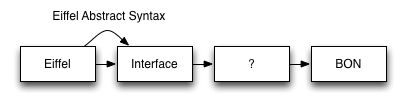
\includegraphics[scale=0.8]{images/BON-extraction-model-2.png}
\caption{BON Extraction Model 2}
\label{fig:bon_extraction_2}
\end{figure}

\paragraph{}
To create the \textsc{bon} representation, a link (the missing link in figure \ref{fig:bon_extraction_2}) between the abstract syntax and the internal representation is needed. Creating a meta-object that instantiates the modeling classes based on the abstract Eiffel syntax provides this functionality. This meta-object will inspect the abstract Eiffel syntax and instantiate the textual \textsc{bon} objects based on the extracted information.

\begin{figure}[H]
\centering
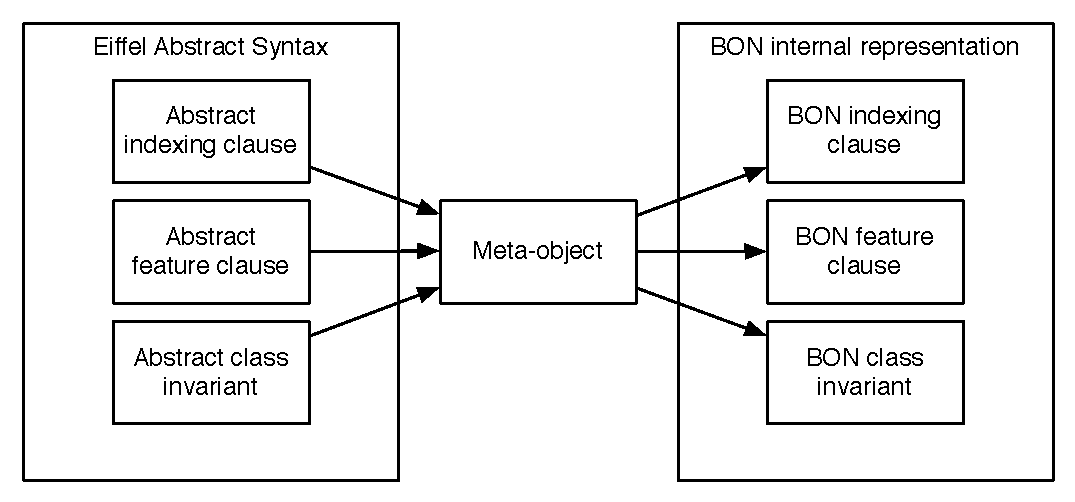
\includegraphics[scale=0.8]{images/metaobject.pdf}
\caption{The function of the \bon{} meta-object}
\label{fig:bon-meta-object}
\end{figure}

The function of the meta-object is convert the abstract Eiffel syntax given by EiffelStudio into the internal \bon{} representation. As it can be seen in figure \ref{fig:bon-meta-object} the meta object extracts the information out of the abstract Eiffel syntax and turns it into its \bon{} counter parts. The meta-object both creates objects for informal and formal specifications.

\begin{figure}[H]
\centering
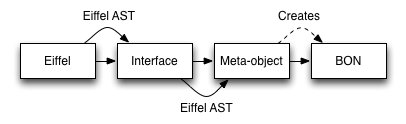
\includegraphics[scale=0.8]{images/BON-extraction-model-3.png}
\caption{BON Extraction Model 3}
\label{fig:bon_extraction_3}
\end{figure}

\paragraph{}
Since each of these \textsc{bon} objects are able to generate textual \textsc{bon} from the information given by the meta-object, the system is now ready to generate \textsc{bon}. However, the textual \textsc{bon} still needs to be handed back to EiffelStudio for it to be displayed to the user.

\subsubsection{From BON to EiffelStudio}
Next step is for the modeling classes to hand back the formatted textual \textsc{bon} to EiffelStudio for it to be shown to the user. To do so either each step needs a reference back to where the textual \textsc{bon} is needed in order to be displayed, or each step needs to be able to receive the result of the following step and hand it back to its predecessor. In the current implementation it has been decided to pass a reference pointing to a decorating object all the way down the \textsc{bon} object structure, such that it is transparent to the creator of the textual \textsc{bon} that it is writing directly to EiffelStudio.

\begin{figure}[H]
\centering
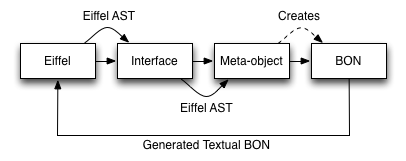
\includegraphics[scale=0.8]{images/BON-extraction-model-4.png}
\caption{BON Extraction Model 4}
\label{fig:bon_extraction_4}
\end{figure}

\subsubsection{Alternatives}
This way of extracting \textsc{bon} from Eiffel has the feel of a visitor pattern, but is not quite the same. This raises the question; why not use a visitor pattern? Had it been the intention to use the \textsc{bon} extractor for multiple languages a visitor pattern would have had its benefits. But since it is a part of EiffelStudio, and therefore only targets the Eiffel language, a visitor pattern would only cause a more cluttered structure. Furthermore it would require all \textsc{bon} generation to be located in one class, namely the visitor class. This would lead to a potentially confusing centralized structure, and in terms of extending the \textsc{bon} generator, would make it harder to locate where to extend the code. There would be both objects holding the data and representing the \textsc{bon} structure and be a central class taking care of handling the information.
\paragraph{}
An alternative solution would be to only have one centralized class taking care of all the generation. This would require less overhead than the implemented solution, since it would remove the need for a meta-object and the need for the MOG-like representation of the \textsc{bon} grammar. This would, however, like the visitor pattern, create a disordered structure with all generation happening in a single class, which would make extension difficult.

\subsection{Design decisions - Deviations from BON}
\label{deviations_from_bon}There are some deviations from the original \textsc{bon} grammar \cite[pp.~352-359]{walden1995}, both in the internal \textsc{bon} representation, but also in the generated textual \textsc{bon}. This section will discuss the most important ones. 

\paragraph{}
\label{part}
The only major difference in the generated \textsc{bon} is the omission of the \textit{part} keyword. There are two uses of \textit{part}. One is that one class in \textsc{bon} can exist over multiple documents. The extractor will never try to split a class up over more than one document, thus this use of the keyword will not be needed. The other is the ability to have partial classes. This feature is seen in some languages (like C\#, \cite{msdn2009}), but since Eiffel does not support partial classes there is no need for it in this implementation. Therefore the \textit{part} keyword is not included in the generated \textsc{bon} nor modeled in the internal representation.

\paragraph{}
Lastly, some elements such as scenario charts and event chart are also not included. Some of these elements were excluded because they only hold semantic value and therefore require the static analysis to gather semantic information from the abstract syntax. Others have been excluded, not because they did not feel relevant or useful for this tool, but because they felt out of scope, such as creation chart. This, however, does not mean that these elements could not be included in future versions of the extractor.
